\chapter*{Introduction}
\chaptermark{Introduction}



% introduzione in cui parliamo di BaseLib/MARTe in modo generale
% presentiamo lo schema logico dopo di che spieghiamo brevemente ogni singola componente

% BaseLib/MARTe �
% software framework, distribuito, component based, supporta diverse arch, diversi OS
BaseLib/MARTe are togheter a complete software framework to run a distributed control code on different architectures and operating systems. BaseLib/MARTe are not only a middleware but include also a collection of different components, i.e. computational blocks. \\

% BaseLib/MARTe �
% rapid design (se ci sono i componenti), fast time to market
A control system is not more than the interconnection of computational blocks, devices that read signals from the environment and then write them out of the digital system. If a digital control system can be completely designed with blocks included in the BaseLib/MARTe library the implementation is straightforward and can require only a couple of hours. \\

% Differenza tra BaseLib e MARTe
The whole project can be logically splitted in BaseLib, MARTe and the components collection. BaseLib offers the basic data structures, an architecture and OS independent API, an object accounting and tracing infrastructure, a serialization and reflection faciliy and all key mechanisms to run a control system; MARTe lets the control algorithm run.

The componets collection is a growing set of algorithmic blocks (GAMs), device drivers adaption blocks (IOGAMs) and device drivers (GACQMs). All the code is written in C/C++. Figure \ref{f:intro:BaseLibMARTe} is a complete schema of the software framework we are going to analyse in this text. \\

\begin{figure}[h!]
 \begin{center}
  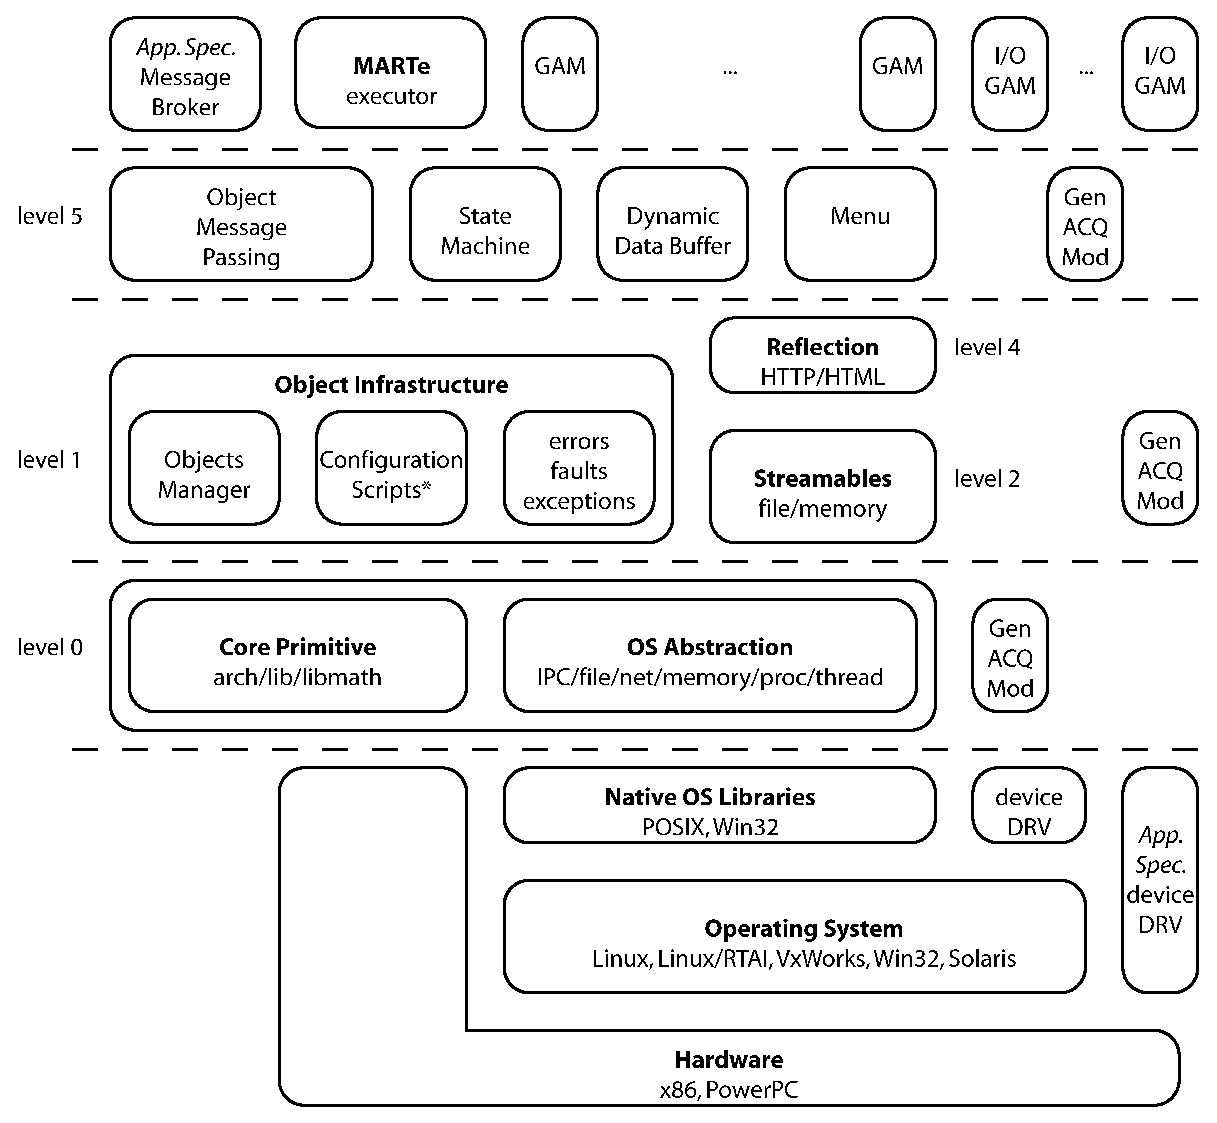
\includegraphics[width=0.63\textwidth]{images/BaseLibMARTe1.eps}
  \caption{BaseLib and MARTe schema}
  \label{f:intro:BaseLibMARTe}
 \end{center}
\end{figure}

The cited Figure highlights the supported operating systems, those are: Microsoft Windows$^\copyright$ 32bit, Linux, Linux/RTAI, Wind River VxWorks$^\copyright$ and Sun Microsystems Solaris$^\copyright$. The supported architectures are: Intel x86 and IBM/Motorola PowerPC (now Freescale), BaseLib/MARTe worked also on SPARC machines but it is not recently tested on. A list of supported I/O and timing devices (ADC and DAC boards) is not available yet. \\


% Posizioniamo BaseLib/MARTe tra i software di controllo come OROCOS
BaseLib/MARTe is a rapid deve lopment control software that can be suitable to automation industry, robot control and manufaturing processes supervision. In those markets we can find other software products, never used in fusion research, those softwares comes from differents experience but most of them lead to the same functionalities and ideas on which BaseLib/MARTe was built. \\

The oldest project we can find on Internet is \textbf{OSACA} (http://www.osaca.org), i.e. Open System Architecture for Controls within Automation systems, focuses on industrial control, is not opensource and probably not manteined yet. There are two government founded project: \textbf{TORERO}, TOtal life cycle web-integrated control design architecture and methodology for distributed control systems in factory automation (http://www.uni-magdeburg.de/iaf/cvs/torero/), and \textbf{OMAC}, the Open Modular Architecture Controller (http://www.isd.mel.nist.gov/projects/). Fully open source university founded projects are: \textbf{OROCOS} (http://www.orocos.org) the Open RObot COntrol Software; \textbf{MCA2} (http://www.mca2.org/) the Modular Controller Architecture (Version 2); \textbf{MICROB} (http://www.robotique.ireq.ca/microb/en/index.html) the Modules Int\'egr\'es pour le Contr\^ole de ROBots and \textbf{OASYS} (http://www-lar.deis.unibo.it/oasys/) the Open source software for industrial Automation and distributed SYstemS (probably part of the TORERO alliance). \\

% saerebbe da spiegare meglio perche
% fondamentalmente perche non e a componenti ma soprattutto e un middleware
The famous \textbf{EPICS} framework (the TANGO framework can be considered as well) doesn't appear in the previous list because it doesn't provide all the basic architectural and design requirement a generic control systems needs to be setup. EPICS, as well as \textbf{CORBA} in the Enterprise Market, is a middleware: it just defines a common protocol to lets different machines (equipped with potentially different OS and processor) communicate. Another middleware used by many automation companies on only Microsoft enabled products is \textbf{OPC} (http://www.opcfoundation.org) the OLE for Process Control, it exploits Microsoft's OLE/COM/DCOM technologies. \\

Various instances of BaseLib/MARTe running in a distributed system can communicate using object messaging, application specific message brokers can also be written to handle 3rd party messages (Figure \ref{f:intro:BaseLibMARTe}). There is an ongoing effort to turn BaseLib/MARTe in an EPICS enabled product. \\



\subsection{Project Organization}
% visione generale del progetto dal punto di vista dello sviluppatore
% diverse entita di codice necessarie i.e. project structure (in future: how to compile)
The whole project is structured in at minimum three packages (directories):
\begin{itemize}
 \item MakeDefaults
 \item BaseLib (or BaseLib2)
 \item MARTe
\end{itemize}

Components (i.e. GAMs) are allotted between the \textit{BaseLib} directory and the \textit{MARTe} directory, other GAMs's directory can be present in your project. The directory \textit{MakeDefaults} group togheter all files to build the software, it supports the Microsoft build system as well as the GNU Makefile utility. The directory \textit{BaseLib} holds all BaseLib files and subdirectories, obviously the directory \textit{MARTe} contains all MARTe files and subdirs, that are presented at the end of the chapter. \\

% il sistema e facile da compilare
% perche tutto il codice lo sviluppiamo noi e non richiede librerie esterne
This directories represent the whole software framework, no external library or software is required, only a working supported Operating System. This means no external dependencies, no dependecies checking and a faster time to a ready to use system. Other projects use differents 3d party libraries and its a pain for a user to put all libraries working togheter.
% in futuro si potrebbero usare librerie esterne 
% la via corretta sarebbe come fa insight che viene distribuito con le librerie che sono state usate
The best solution in this sense is to distribuite the 3d party libraries togheter with the software package, this option can be considered in the future to speed up upgrades of the BaseLib/MARTe code (imagine to add XML support). \\

% si puo mettere qualche numero riguardo al numero di classi e interfaccie presenti rispetto al
% numero di classi che ci sono in altri framework a componenti

To compile the whole project two steps are needed: first you must compile BaseLib and then it is possible to build MARTe. When the libraries are ready you need a configuration file to see something running.



\subsection{Component Object Model}
% component object model similarita con altri progetti (OROCOS) [COM, Java]
% patterns, che design patterns sono stati utilizzati
Most software products nowadays utilize several design patterns; BaseLib/MARTe explicitly uses the Container (Composite), the Iterator, Command and State design patterns (last threes of these are considered by the GAMMA behavioral patterns). Also the Observer, Prototype, Adapter, Bridge and Decorator design patterns are used but the implementation comes naturally, without any previous class's design.

% component object model - component oriented programming
% si � puntato sullo sviluppo COM cioe via interfaccia
Instead, the development of BaseLib/MARTe was done following the Component Oriented Programming practice (well known as Component Object Model). Following such paradigm all communications between objects use a well known interface, the source code is infact rich of interface definitions. \\

% component oriented programming - connection oriented programming (GAM)
% di solito un singolo comoponente = un obj --> GAM
BaseLib/MARTe is built on different components, these usually lead to be developed in single classes, i.e. one component is implemented within one C++ class. These is especially true for the computational blocks that realize a control system from an algorithmic point of view.
A control system can be first designed using a Block Diagram Modeller IDE (Matlab Simulink$^\copyright$, Scicos, NI LabView$^\copyright$ or Ptolemy/Kepler) and then converted for execution in BaseLib/MARTe. Each computational block of the diagram will be mapped to a software component called Generic Application Module (GAM); GAMs are then connected via a memory bus component that offers some interfaces but also requires to be compliant to other interfaces. The definition of incoming and outcoming interfaces is usually referred to Connection Oriented Programming and is a particular programming style that is especially useful when aiming for Component Oriented Programming. Figure \ref{f:intro:GAMComponent} show how connection can be setup between components.

\begin{figure}[h!]
 \begin{center}
  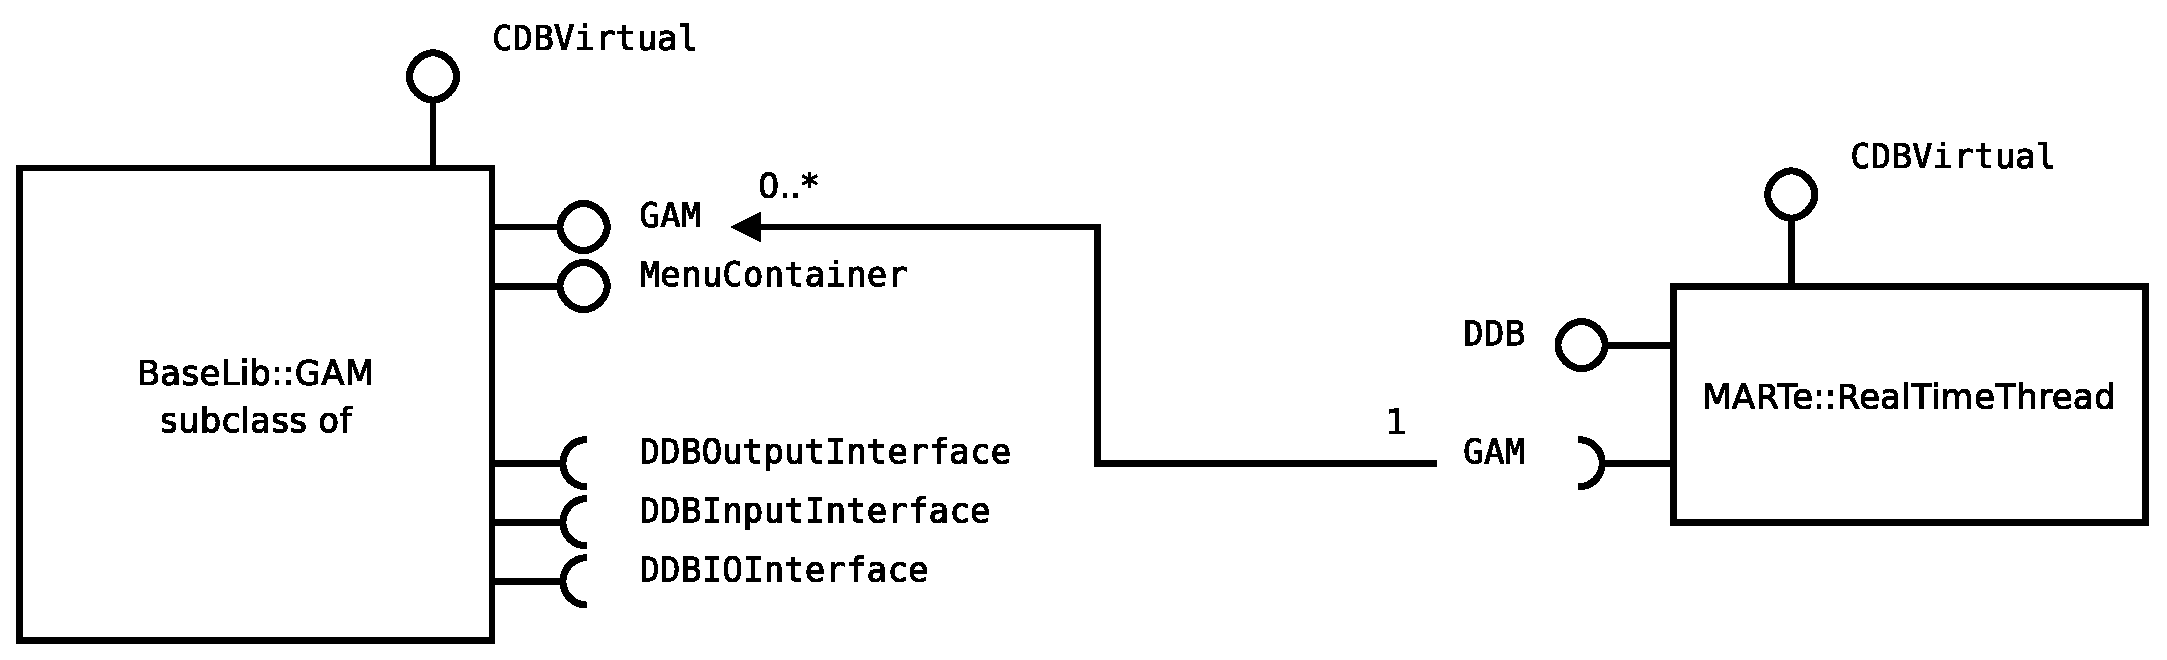
\includegraphics[width=0.77\textwidth]{images/GAMComponent.eps}
  \caption{Components connections in BaseLib/MARTe}
  \label{f:intro:GAMComponent}
 \end{center}
\end{figure}

Such Figure points out the connection between a \texttt{MARTe::RealTimeThread} component and many \texttt{BaseLib::GAM} subclass components, note the multiplicities at each ends of the association.
A \texttt{BaseLib::GAM} subclass component, or simply a GAM, holds receptacles for \texttt{DDBInputInterface}, \texttt{DDBOutputInterface} and \texttt{DDBIOInterface}. Such interfaces lets
a GAM produce and consume datas on the common memory bus called Dynamic Data Buffer (DDB). The \texttt{CDBVirtual} interface lets components load and save its configuration from and to a configuration file (in a human readable format). The \texttt{MenuContainer} interface lets components export a menu user interface to enable users to see and change component's parameter in real time. \\


% i componenti mono source sono le GAM - il resto del codice segue la programmazione OO
% e i componenti non sono esplicitamente definiti
Most of the code in the project that doesn't extends or doesn't implement a GAM is infrastructural and lets GAMs load, connect between them, run and save is state (persistence), the exception is MARTe that is a scheduling entity of all GAMs. Figure \ref{f:intro:BaseLibMARTe3D} illustrate this concept. Note that this doesn't mean that only GAMs are components, all the software is structured using the Component Object Model. \\

\begin{figure}[h!]
 \begin{center}
  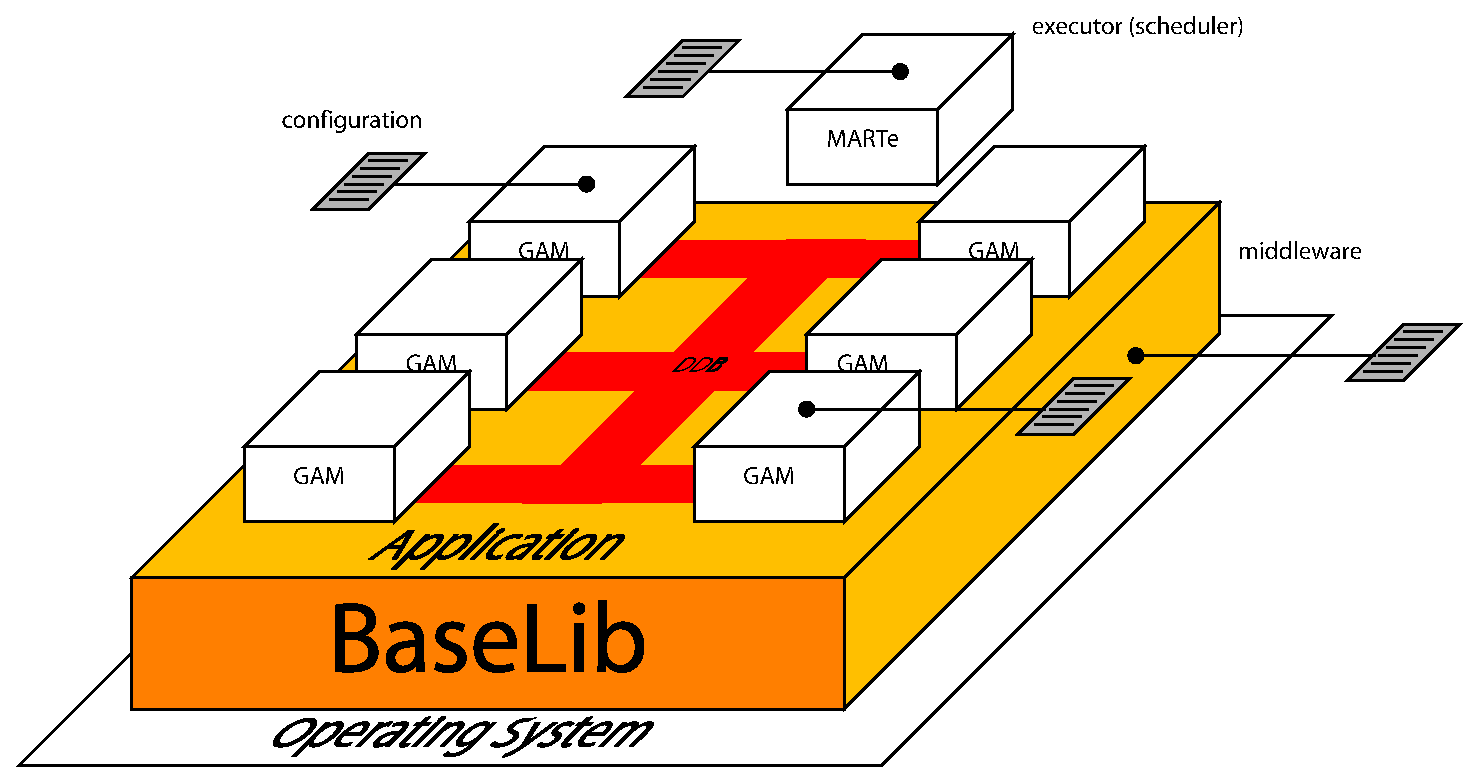
\includegraphics[width=0.77\textwidth]{images/BaseLibMARTe3D.eps}
  \caption{BaseLib and MARTe schema in 3D}
  \label{f:intro:BaseLibMARTe3D}
 \end{center}
\end{figure}

Referring to the same picture is simple to understand what a user application running in BaseLib/MARTe is: \textbf{a collection of interconnected components initialised via a configuration file}. \\

If components for your control system application are just written no understanding of the entire software framework is needed and also no programming skills are required because you can implement the control system using only a human readable/writable configuration file (similar to the Microsoft's \texttt{ini} files). \\



\subsection{Reflection, Persistence, Garbage Collection and Messages}

A big difference between the most used C object oriented version (C++) and the Sun Object Oriented language Java is the lack of reflection, persistence (serialization) and garbage collection of the former.
These capabilities enable Java to manage every aspect of objects lifecycle, from the creation to the destruction providing also a runtime inspection. Both C++ and Java supply runtime introspection (C++ by means of RTTI). \\


Smalltalk and Objective C languages have built-in reflection besides introspection; such languages add Object Messaging. To get an object to do something, you send it a message telling it to apply a method or to do an activity. Programming by messages instead using method calls ensure inter-thread communication safety without holding locks. \\


BaseLib/MARTe as a C/C++ framework supplies to the user a complete solution that introduce in C/C++ language an esay to use reflection, persistence, garbage collection and object messaging, all those capability work on different compilers and different operating systems.
Looking back at Figure \ref{f:intro:BaseLibMARTe} there is a block named \textit{Object Infrastructure}, this block is deepened in Figure \ref{f:intro:BaseLibOI} and implements the core functionalities for object handling and inspection.
Those object level features are not common to a component based software that usually takes into account component-alike properties (this is the behavior of the previous cited OROCOS control framework). Such added capabilities add at minimum another level of complexities to the schema in Figure \ref{f:intro:BaseLibMARTe3D} where for example there is no object message loop. \\

\begin{figure}[h!]
 \begin{center}
  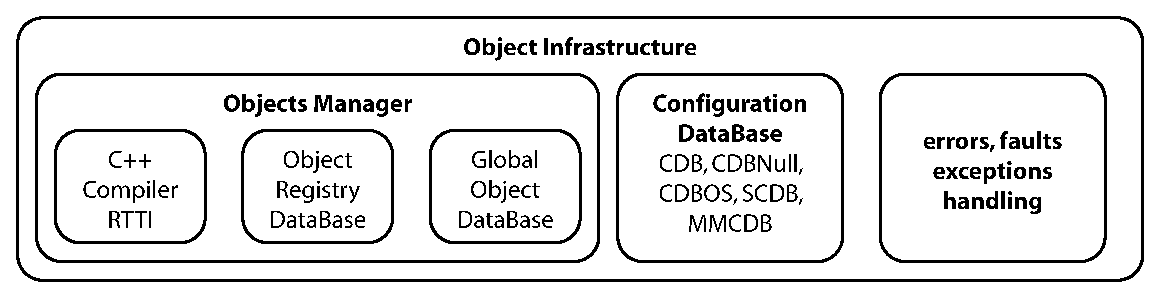
\includegraphics[width=0.77\textwidth]{images/BaseLibOI.eps}
  \caption{BaseLib Object Infrastructure}
  \label{f:intro:BaseLibOI}
 \end{center}
\end{figure}

Figure \ref{f:intro:BaseLibOI} highlights the different entity componing the \textit{Object Infrastructure}: an object manager built on top of the C++'s compiler RTTI, an Object Registry DataBase (ORDB), i.e. a list of all objects type currently loaded in the system; a Global Object DataBase (GODB), i.e. a list of all currently instantiated objects; a configuration utility (the CDB) that lets load and save object's attributes (i.e. implement the serialization) and an error management unit. \\

% come si arriva alla serializzazione
% late binding implicito
Exploiting the RTTI facility and language macros the ORDB and the GODB implement reflection and garbage collection. Garbage collection is done by refernce counting. External live reflection capability is offered via an HTTP server at highers level (many industrial boards nowadays lets the user inspect it via a web browser).

The CDB exploiting ORDB and GODB adds serialization. The serialization in BaseLib/MARTe is done by each object, i.e. only the single object is aware of its attributes (or parameters). The serialization is not done on human unreadable format but in a simple format that lets a user write it's own file, a configuration file is a human readable serialization of objects. A whole control system can be written using only a single configuration file without a single line of C/C++.

% object messaging
Object Messaging is achieved by the \textit{Object Message Passing} infrastructure in a higher level of the framework (have a look at Figure \ref{f:intro:BaseLibMARTe}). This entity will be integrated in the Object Infrastructure. \\



%\subsubsection{Code Conventions}
% scelte implementative del codice
% classi inline, problema delle DLL
% le classi vengono scritte con il codice in C per permettere alle DLL di essere compilate in modo che si possa fare un late binding
% il motivo in realta per il momento mi e oscuro. cmq o centra con le DLL oppure centra con il supporto a diversi compilatori.
% in pratica molte classi hanno i loro metodi implementati come inline che richiamano funzioni C friend
% invece di avere comuni metodi implementati nel file cpp con la dichiarazione classe::nome



% BaseLib states
% BaseLib organization (current version)
\section{BaseLib}
BaseLib is a library, i.e. a collection of codes. BaseLib relay on very few global data structures loaded at initialization time, it is the user that loads the framework via a function call that invoke all the startup process.

The startup process (CREATION state) of BaseLib reads a configuration file (also in memory) then creates all objects in such file with the correct attribute's values (exploiting serialization). If the creation finishes without any problem the framework is in the RUNTIME state, in this state MARTe is running. If MARTe chooses to exit move all the system in the DELETION state, the last state before application end. In each state BaseLib can moves to the ERROR state. The whole BaseLib state transitions are depicted in Figure \ref{f:intro:BaseLibStates}; BaseLib doesn't know about its internal state unless it is in ERROR, BaseLib' states are just an abstraction to understand its behaviour. \\

\begin{figure}[h!]
 \begin{center}
  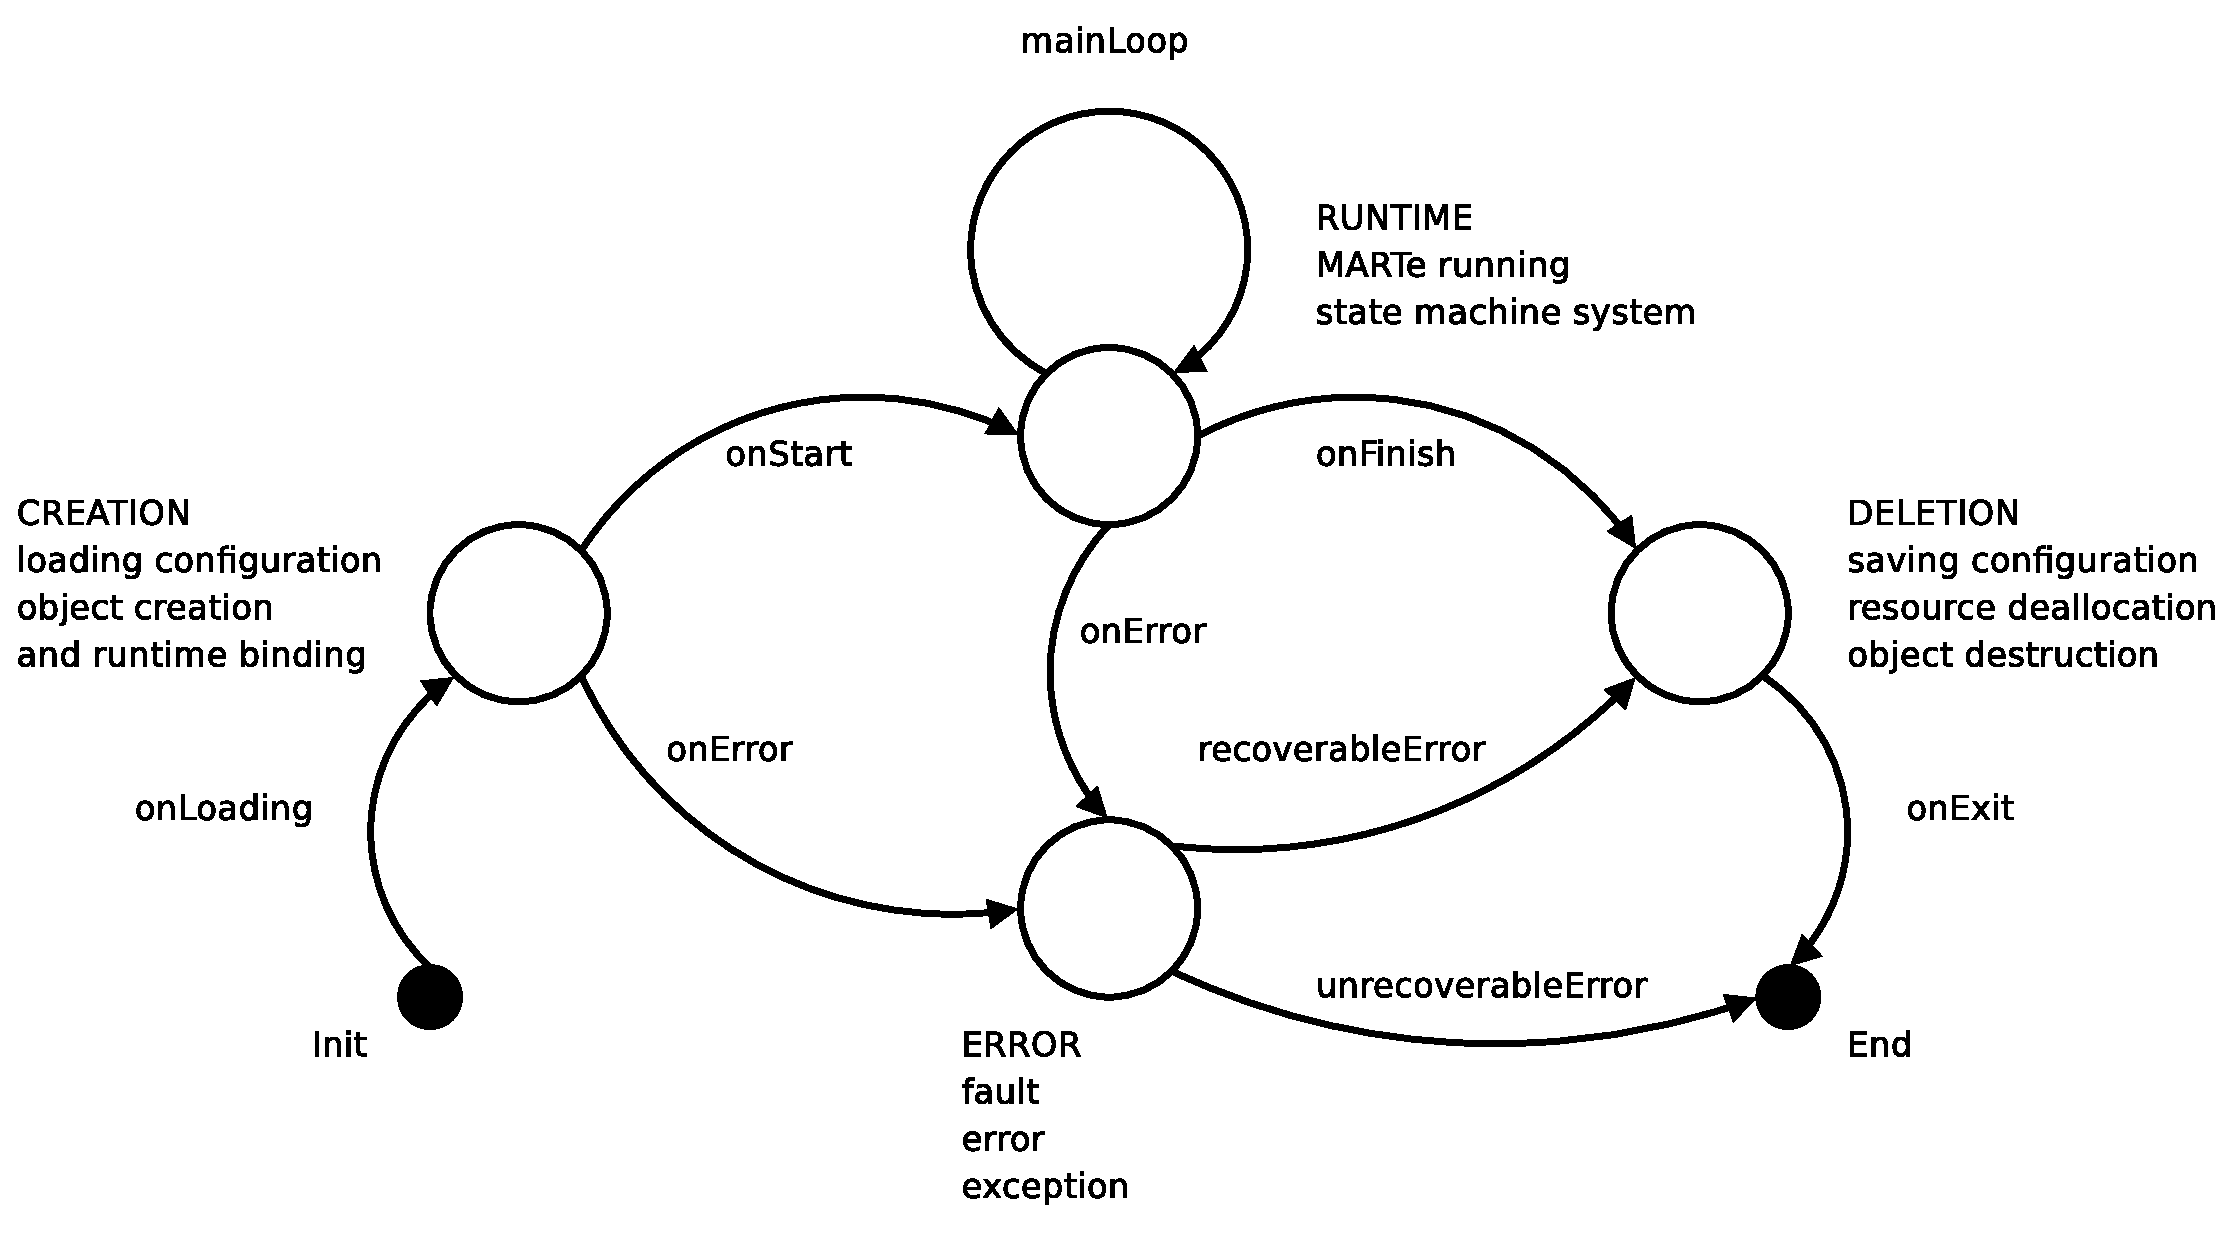
\includegraphics[width=0.77\textwidth]{images/BaseLibStates.eps}
  \caption{BaseLib's main states}
  \label{f:intro:BaseLibStates}
 \end{center}
\end{figure}

BaseLib's core source code is partitioned right now in seven different directories, each one is a \textit{level} starting from \textit{level0} up to \textit{level6}. Code in a directory within an higher \textit{level} depends on code in low \textit{level} directories like in an hierarchy relationship.

BaseLib contains also other code, it holds a collection of GAMs (common and wide used ones), some testing applications and useful debugging and logging tools. All that in four different directories: \textit{LoggerService}, \textit{GAMs}, \textit{BaseLibTests}, \textit{BaseLibTools}.

In this work only \textit{level} directories will be analised. At the end of reading it will be easy to understand that the subdivision by compilation dependence doesn't ease the understanding of the project (also if can be a good choice for debugging the project). Table \ref{T:levels} summarizes which component it is possible to find in each level. The CDB's code for example is spreaded between \textit{level0}, \textit{level1}, \textit{level3} and \textit{level6}. Same work must be done in these direction to ease code comprehension and modularity. \\

\begin{table}[!ht]
 \begin{center}
  \begin{tabular}{|l|l|}
\hline
\textbf{level 0} & OS Abstraction\\
 & Core Primitives \\
\hline
\textbf{level 1} & Garbage Collection \\
 & ObjectRegistryDataBase (ORDB) \\
 & GlobalObjectDataBase (GODB) \\
 & ConfigurationDataBase (CDB) \\
\hline
\textbf{level 2} & streams \\
 & ConfigurationDataBase (CDB) \\
\hline
\textbf{level 3} & ConfigurationDataBase (CDB) \\
 & ConfigurationDataBase OutputStream (CDBOS) \\
 & parser \\
\hline
\textbf{level 4} & HTTP, HTML protocol libraries\\
\hline
\textbf{level 5} & Dynamic Data Buffer (DDB)\\
 & Generic Acquisition Module (GAM) \\
 & Messages \\
 & State Machine \\
 & Menu \\
\hline
\textbf{level 6} & Memory Mapped CDB (MMCDB)\\
 & maths objects \\
\hline
  \end{tabular}
 \caption{BaseLib levels}
 \label{T:levels}
 \end{center}
\end{table}


% MARTe states
% MARTe organization (current version)
\section{MARTe}
MARTe library is a collection of GAMs, IOGAMs, GACQMs and an executor (or dispatcher). Such executor is a thread that run consecutively a set of GAMs and IOGAMs; the set that is currently running depends on the state of the plant system and the controller machine. There are basically four sets: \textit{initialising}, \textit{offline}, \textit{online} and \textit{safety}. In Figure \ref{f:intro:MARTeStates} the states of the plant system are depicted; usually the \textit{initialising} set is executed only during the INIT state, the \textit{online} set is executed during PREPULSE, PULSE and POSTPULSE; \textit{offline} set is executed in IDLE and WAITINGPRE states. When some error occurs the currently running set is substitued with the \textit{safety} set. \\

\begin{figure}[h!]
 \begin{center}
  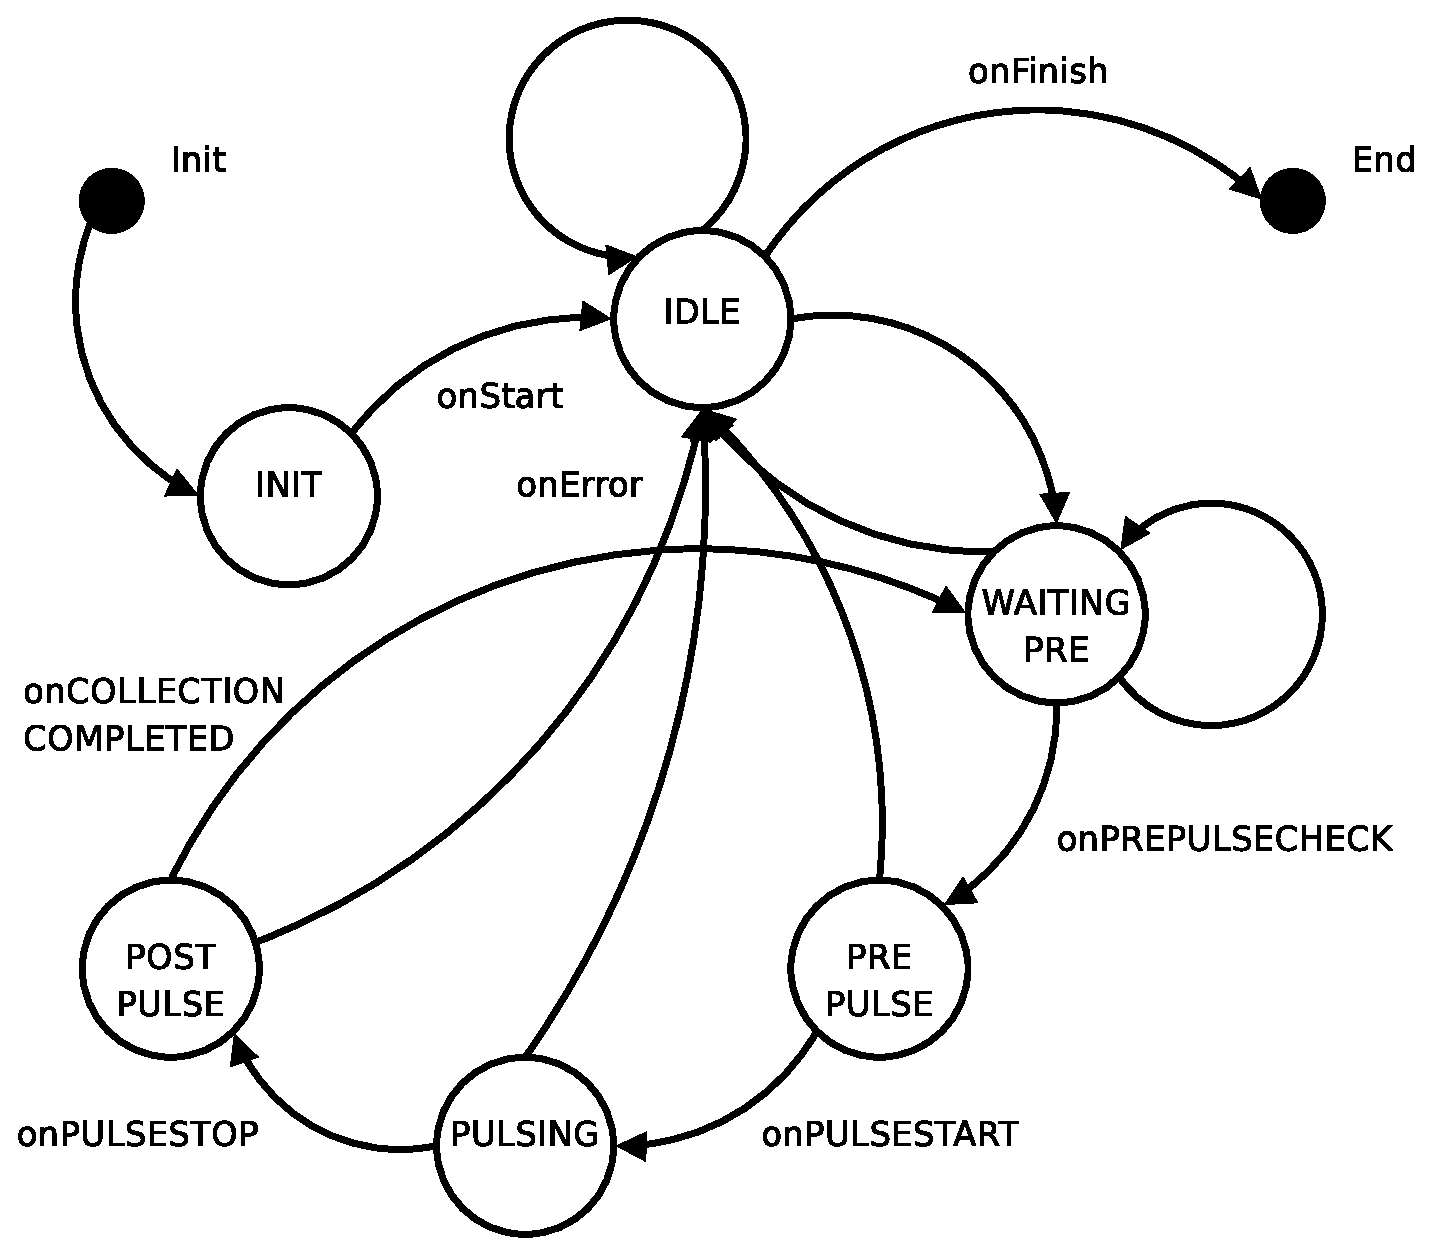
\includegraphics[width=0.50\textwidth]{images/MARTeStates.eps}
  \caption{MARTe States}
  \label{f:intro:MARTeStates}
 \end{center}
\end{figure}

MARTe originates as the first application built on BaseLib library. Some components, like the \textit{RealTime Thread} (the executor), were added because not in BaseLib, MARTe is also the configuration file that request the instantiation of a precise set of components. Figure \ref{f:intro:MARTe} depict the different componets MARTe require to be instantiated.

\begin{figure}[h!]
 \begin{center}
  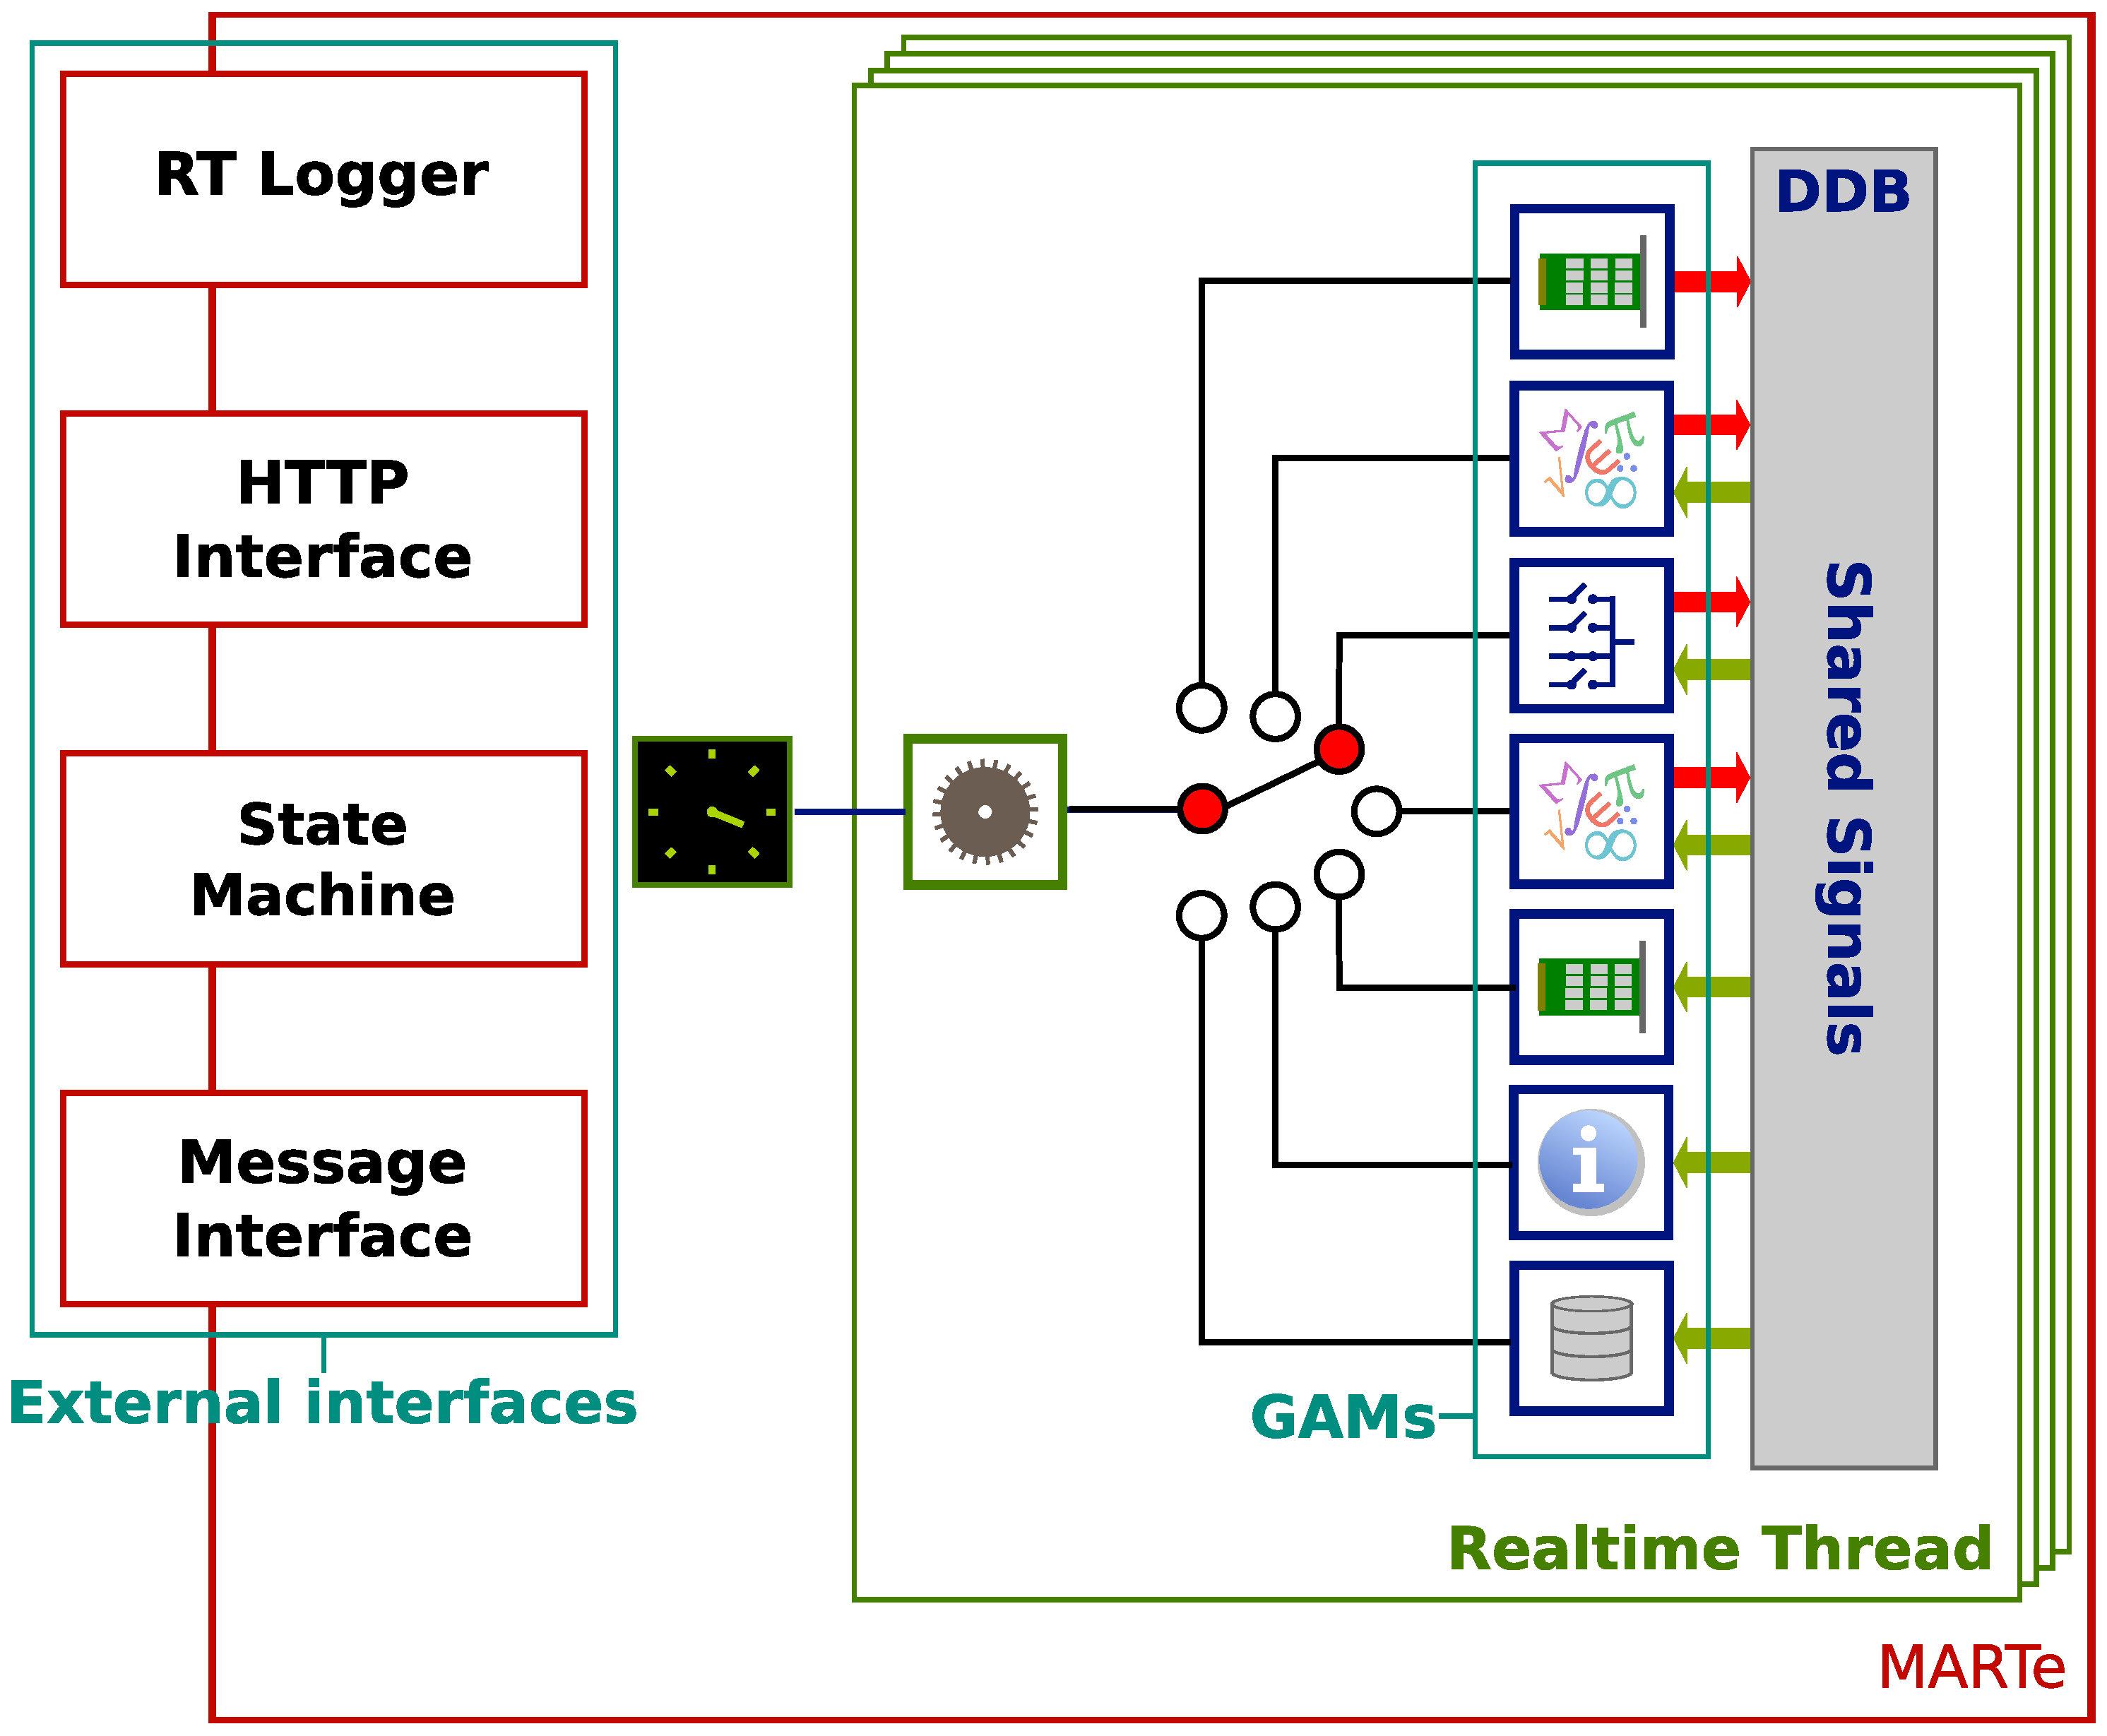
\includegraphics[width=0.48\textwidth]{images/MARTeComponents.eps}
  \caption{MARTe Components}
  \label{f:intro:MARTe}
 \end{center}
\end{figure}

In such Figure there are at least three different components that come from BaseLib: the \textit{HTTP server}, the \textit{Messaging} infrastructure and an \textit{external state machine} that communicate with the internal one. In the Figure is not depicted the communication library that connects MARTe to plant system rendering the application a part of the whole distributed system. The communication library is included in MARTe, right now there is only CODASLib that supports the JET communication protocol; forthcoming libraries will be MDSplusLib and EPICSLib.

\begin{table}[!ht]
 \begin{center}
  \begin{tabular}{|l|l|}
\hline
 \textbf{MARTeSupportLib} & \\
\hline
 \textbf{GAMs} & EventCollection, WaveformCollection, DataCollection \\
 & WebStatistics, Statistics \\
 & Hysteresis, Noise, CurrentControl \\
\hline
 \textbf{IOGAMs} & ATCA, MPV956, MPV922 \\
 & ForeHE, Interphase, LinuxSocket (UNIX), WinSock \\
 & WinTimer, LinuxTimer (UNIX), VxWorksTimer, HRT \\
\hline
 \textbf{CODASLib} & \\
 \textbf{MDSplusLib}* & \\
 \textbf{EPICSLib}* & \\
\hline
  \end{tabular}
 \caption{MARTe directory tree}
 \label{T:trees}
 \end{center}
\end{table}


\section{Remarks}
TODO\\


